\chapter{Ықтималдылық}

\index{ықтималдылық}

\key{Ықтималдылық} -- оқиғаның қаншалықты 
мүмкін болатынын көрсететін
$0$ мен $1$ арасындағы нақты сан. Егер оқиға
белгілі болатын болса, онда ықтималдылығы 1,
ал оқиға мүмкін емес болса,
онда ықтималдылығы 0 болады. Оқиғаның ықтималдылығы 
$P(\cdots)$ түрінде белгілінеді, мұндағы үш нүкте оқиғаны көрсетеді.

Мысалы, ойын сүйегін лақтыратын болсақ,
нәтижесі $1$ мен $6$ арасындағы бүтін сан
және әр нәтиженің ықтималдылығы $1/6$ болады.
Өрнек ретінде төмендегі ықтималдылықтарды есептей 
аламыз:

\begin{itemize}[noitemsep]
\item $P(\textrm{''нәтиже 4 болады''})=1/6$
\item $P(\textrm{''нәтиже 6 болмайды''})=5/6$
\item $P(\textrm{''нәтиже жұп сан''})=1/2$
\end{itemize}

\section{Есептеу}

Оқиғаның ықтималдылығын есептеу үшін комбинаториканы 
қолдануымызға болады немесе оқиғаны тудыратын үдерісті симуляциялай аламыз.
Өрнек ретінде араластырылған карта колодасынан мәні бірдей үш картаны
алып шығу ықтималдылығын есептейік.
(мысалы $\spadesuit 8$, $\clubsuit 8$ және $\diamondsuit 8$).

\subsubsection*{1-әдіс}

Ықтималдылықты есептеу үшін келесі формуланы қолдануымызға болады:

\[\frac{\textrm{қажет нәтижелер саны}}{\textrm{жалпы нәтижелер саны}}.\]

Бұл есепте қажет нәтижелер -- карталардың мәндері 
бірдей болған жағдай. Ондайдың $13 {4 \choose 3}$ жолы бар:
картаның мәніне $13$ мүмкіндік бар және
әр санға $4$ түстен $3$ түсті алу үшін ${4 \choose 3}$ жол бар.

Жалпы нәтижелердің саны -- ${52 \choose 3}$:
біз 52 карта ішінен 3 карта аламыз. Осылайша
оқиғаның ықтималдылығы 

\[\frac{13 {4 \choose 3}}{{52 \choose 3}} = \frac{1}{425}.\]

\subsubsection*{2-әдіс}

Ықтималдылықты есептеудің басқа жолы --
оқиғаны тудыратын үдерісті симуляциялау.
Бұл мысалда біз үш картаны алуымыз керек,
демек үдеріс 3 қадамнан тұрады. 
Біз үдерістің әрбір қадамы сәтті болуын талап етеміз.

Ешқандай шектеу қойылмағандықтан, бірінші картаны алу әрдайым сәтті болады. Екінші
картаны алу $3/51$ ықтималдылықпен сәтті болады,
өйткені бізде 51 карта қалады және 3-уі 
бірінші картадағыдай мәнге ие болады. Дәл солай
үшінші қадам $2/50$ ықтималдылықпен сәтті болады.

Толық үдерістің сәтті болуының ықтималдылығы 

\[1 \cdot \frac{3}{51} \cdot \frac{2}{50} = \frac{1}{425}.\]

\section{Оқиғалар}

Ықтималдылық теориясында оқиғаны жиын ретінде көрсетуге болады
\[A \subset X,\]
мұнда $X$ барлық нәтижелерді қамтиды және
$A$ -- нәтижелердің ішжиыны.
Мысалы, ойын сүйегін лақтырған кезде, нәтижелер төмендегідей болады:
\[X = \{1,2,3,4,5,6\}.\]
Мысалы, ''нәтиже жұп сан'' деген оқиғаға сәйкес жиын
\[A = \{2,4,6\}.\]

Әр $x$ нәтижеге $p(x)$ ықтималдылығын белгілейік.
Онда $A$ оқиғасының ықтималдылығы $P(A)$ нәтижелердің 
ықтималдылықтарының қосындысы ретінде төмендегі формула
арқылы есептеуге болады:
% Each outcome $x$ is assigned a probability $p(x)$.
% Then, the probability $P(A)$ of an event
% $A$ can be calculated as a sum
% of probabilities of outcomes using the formula
\[P(A) = \sum_{x \in A} p(x).\]
Мысалы, ойын сүйегін лақтырған кезде,
әр $x$ нәтижеге $p(x)=1/6$ сәйкес келеді,
демек ''нәтиже жұп сан'' оқиғасының
ықтималдылығы \[p(2)+p(4)+p(6)=1/2.\]. 

$X$-тің барлық нәтижелерінің ықтималдылықтарының қосындысы
1 болу керек, яғни $P(X)=1$.

Ықтималдылық теориясындағы оқиғалар жиын болғандықтан,
біз оған қарапайым жиын операцияларын қолдана аламыз:  

\begin{itemize}
\item $\bar A$ деп $A$-ға \key{толықтыру}
оқиғасын белгілейді. Мысалы ойын сүйегін лақтырған кезде,
$A=\{2,4,6\}$ оқиғасына толықтыру оқиғасы 
$\bar A = \{1,3,5\}$ болады. 
\item $A \cup B$ деп $A$ мен $B$ оқиғаларының \key{біріктіруін}
белгілейді. Мысалы $A=\{2,5\}$ және 
$B=\{4,5,6\}$ оқиғаларының біріктіруі 
-- $A \cup B = \{2,4,5,6\}$. 
\item $A \cap B$ деп $A$ мен $B$ оқиғаларының \key{қиылысуын}
белгілейді. Мысалы $A=\{2,5\}$ және $B=\{4,5,6\}$
оқиғаларының қиылысуы –– $A \cap B = \{5\}$.
\end{itemize}

% \item The \key{complement} $\bar A$ means
% ''$A$ does not happen''.
% For example, when throwing a dice, 
% the complement of $A=\{2,4,6\}$ is
% $\bar A = \{1,3,5\}$.
% \item The \key{union} $A \cup B$ means
% ''$A$ or $B$ happen''.
% For example, the union of
% $A=\{2,5\}$
% and $B=\{4,5,6\}$ is
% $A \cup B = \{2,4,5,6\}$.
% \item The \key{intersection} $A \cap B$ means
% ''$A$ and $B$ happen''.
% For example, the intersection of
% $A=\{2,5\}$ and $B=\{4,5,6\}$ is
% $A \cap B = \{5\}$.


\subsubsection{Толықтыру}

$\bar A$ толықтырудың ықтималдылығы келесі формула
арқылы есептеледі:
\[P(\bar A)=1-P(A).\]

Берілген есепті толықтыруларды пайдаланып қарама-қарсы есепті 
шешу тәсілі арқылы оңай шешуге болады.
Мысалы, 10 рет ойын сүйегін лақтырған кезде 
6 санын кем дегенде бір мәрте көруіміздің ықтималдылығы: 
\[1-(5/6)^{10}.\]
Бұл жердегі $5/6$ -- бір лақтырыстың нәтижесі 6 болмауының, ал $(5/6)^{10}$ -- 10 лақтырыстың ешқайсысы 6 болмауының ықтималдылығы. 
Осының толықтыруы -- берілген есептің жауабы.

\subsubsection{Біріктіру}

$A \cup B$ біріктіруінің ықтималдылығын төмендегі 
формула арқылы есептеуге болады:
\[P(A \cup B)=P(A)+P(B)-P(A \cap B).\]
Мысалы ойын сүйегін лақтырған кезде,
\[A=\textrm{''нәтиже жұп сан''}\] оқиғасы 
мен 
\[B=\textrm{''нәтиже 4-тен кем''}\] оқиғаларының
біріктіруі –– \[A \cup B=\textrm{''нәтиже жұп сан немесе 4-тен кем''},\]
және оның ықтималдылығы -- 
\[P(A \cup B) = P(A)+P(B)-P(A \cap B)=1/2+1/2-1/6=5/6.\]

Егер $A$ мен $B$ оқиғалары \key{қиылыспайтын}, яғни
$A \cap B$ бос болса, 
$A \cup B$ оқиғасының ықтималдылығы --

\[P(A \cup B)=P(A)+P(B).\]

\subsubsection{Шартты ықтималдылық}

\index{шартты ықтималдылық}

\key{Шартты ықтималдылық}
\[P(A | B) = \frac{P(A \cap B)}{P(B)}\] --
$B$ орын алғанда $A$ оқиғасының ықтималдылығы.
$A$–ның ықтималдылығын есептегенде,
біз тек $B$–ға тиесілі нәтижелерді қарастырамыз. 

Алдыңғы жиындарды қолдансақ,
\[P(A | B)= 1/3,\]
себебі $B$-ның нәтижелері 
$\{1,2,3\}$, және олардың біреуі ғана
жұп. Бұл егер нәтиже $1 \ldots 3$ арасында болса, 
нәтиженің жұп болуының ықтималдылығын білдіреді. 

\subsubsection{Қиылысу}

\index{тәуелсіздік}

Шартты ықтималдылықты қолданып,
$A \cap B$ қиылысуының ықтималдылығын 
келесі формула арқылы есептеуге болады:
\[P(A \cap B)=P(A)P(B|A).\]
Егер 
\[P(A|B)=P(A) \hspace{10px}\textrm{және}\hspace{10px} P(B|A)=P(B),\]
болса, $A$ мен $B$ оқиғалары \key{тәуелсіз} болады. Бұл $B$-ның орын алуы $A$-ның ықтималдылығына 
және $A$-ның орын алуы $B$-ның ықтималдылығына 
еш әсер бермейтінін білдіреді. 
Бұл жағдайдағы қиылысудың ықтималдылығы --
\[P(A \cap B)=P(A)P(B).\]
Мысалы, колодадан картаны алғанда,
\[A = \textrm{''картаның түсі жүрек''}\]
және
\[B = \textrm{''картаның мәні 4''}\]
екенін көреміз. Демек 
\[A \cap B = \textrm{''картаның мәні 4 және түсі жүрек''}\] оқиғасы
\[P(A \cap B)=P(A)P(B)=1/4 \cdot 1/13 = 1/52\] ықтималдылықпен
орын алады. 

\section{Кездейсоқ шамалар}

\index{кездейсоқ шамалар}

\key{Кездейсоқ шама} -- кездейсоқ үдерістен құрылған
мән. Мысалы, екі ойын сүйегін лақтырған кезде, 
келесі кездейсоқ шаманы анықтауға болады:
\[X=\textrm{''нәтижелердің қосындысы''}.\]
Егер нәтижелер $[4,6]$ болса (яғни бірінші лақтырыстың
нәтижесі төрт және екінші лақтырыстың нәтижесі алты), 
онда $X$-тің мәні 10 болады. 

$P(X=x)$ деп $X$ кездейсоқ шаманың 
$x$-ке тең болуының ықтималдығы деп белгілейміз. 
Мысалы, екі ойын сүйегін лақтырған кезде, 
$P(X=10)=3/36$, өйткені жалпы нәтижелердің саны 
36 және қосындысы 10 болатын 3 нәтиже бар: 
$[4,6]$, $[5,5]$ және $[6,4]$.


\subsubsection{Математикалық күтім}

\index{математикалық күтім}

\key{Математикалық күтім} $E[X]$ -- $X$
кездейсоқ айнымалының орташа мәні. 
Математикалық күтімді қосындылар арқылы 
есептеуге болады: 
\[\sum_x P(X=x)x,\]
мұндағы $x$ барлық $X$-тің мәндерінен өтіп шығады. 

Мысалы, ойын сүйегін лақтырған кездегі 
нәтиженің математикалық күтімі -- 
\[1/6 \cdot 1 + 1/6 \cdot 2 + 1/6 \cdot 3 + 1/6 \cdot 4 + 1/6 \cdot 5 + 1/6 \cdot 6 = 7/2.\]

Математикалық күтімнің пайдалы қасиеті --
\key{сызықтық}. Ол 
$E[X_1+X_2+\cdots+X_n]$ қосындысы 
әрдайым 
$E[X_1]+E[X_2]+\cdots+E[X_n]$ қосындысына тең дегенді білдіреді. 
Бұл формула егер кездейсоқ шамалар өзара тәуелді болса
да орындалады. 

Мысалы екі ойын сүйегін лақтырған кезде,
математикалық күтім --
\[E[X_1+X_2]=E[X_1]+E[X_2]=7/2+7/2=7.\]

Енді басқа есепті қарастырайық:
$n$ доп $n$ қорапқа кездейсоқ салынған. 
Біздің тапсырмамыз -- бос қораптар санының 
математикалық күтімін есептеу. Әр доп 
кез келген қорапқа бірдей ықтималдылықпен салына алады.
Мысалы, егер $n=2$ болса, нәтижелер төмендегідей болуы мүмкін:
\begin{center}
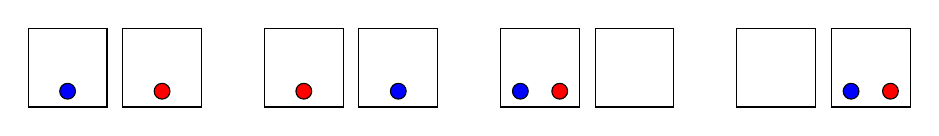
\begin{tikzpicture}
\draw (0,0) rectangle (1,1);
\draw (1.2,0) rectangle (2.2,1);
\draw (3,0) rectangle (4,1);
\draw (4.2,0) rectangle (5.2,1);
\draw (6,0) rectangle (7,1);
\draw (7.2,0) rectangle (8.2,1);
\draw (9,0) rectangle (10,1);
\draw (10.2,0) rectangle (11.2,1);

\draw[fill=blue] (0.5,0.2) circle (0.1);
\draw[fill=red] (1.7,0.2) circle (0.1);
\draw[fill=red] (3.5,0.2) circle (0.1);
\draw[fill=blue] (4.7,0.2) circle (0.1);
\draw[fill=blue] (6.25,0.2) circle (0.1);
\draw[fill=red] (6.75,0.2) circle (0.1);
\draw[fill=blue] (10.45,0.2) circle (0.1);
\draw[fill=red] (10.95,0.2) circle (0.1);
\end{tikzpicture}
\end{center}
Бұл жағдайда қораптың бос болуының математикалық
күтімі --
\[\frac{0+0+1+1}{4} = \frac{1}{2}.\]
Жалпы жағдайда қораптың бос болуының ықтималдылығы --
\[\Big(\frac{n-1}{n}\Big)^n,\]
себебі оған ешқандай доп салынбауы керек.
Осылайша, сызықтық қасиетті қолданған кездегі 
бос қораптардың санының математикалық күтімі --
\[n \cdot \Big(\frac{n-1}{n}\Big)^n.\]

\subsubsection{Үлестірім}

\index{үлестірім}

$X$ кездейсоқ шаманың \key{үлестірімі}
$X$-те бола алатын барлық мәндерінің ықтималдылығын
көрсетеді. Үлестірім $P(X=x)$ мәндерінен тұрады. 
Мысалы, төменде екі ойын сүйегін лақтырған кездегі 
нәтижелердің қосындысының үлестірімі берілген:
\begin{center}
\small {
\begin{tabular}{r|rrrrrrrrrrrrr}
$x$ & 2 & 3 & 4 & 5 & 6 & 7 & 8 & 9 & 10 & 11 & 12 \\
$P(X=x)$ & $1/36$ & $2/36$ & $3/36$ & $4/36$ & $5/36$ & $6/36$ & $5/36$ & $4/36$ & $3/36$ & $2/36$ & $1/36$ \\
\end{tabular}
}
\end{center}

\index{бірқалыпты үлестірім}

\key{Бірқалыпты үлестірімде} $X$ кездейсоқ шамасында 
$n$ мүмкін болатын $a,a+1,\ldots,b$ мәндері бар және әр мәнінің 
ықтималдылығы $1/n$. Мысалы ойын сүйегін лақтырған кезде 
$a=1$, $b=6$ және әр $x$ мәніне $P(X=x)=1/6$ орындалады.

Бірқалыпты үлестірімдегі $X$ мәнінің математикалық күтімі ––
\[E[X] = \frac{a+b}{2}.\]

\index{Биномдық үлестірім}
\key{Биномдық  үлестірімде} $n$ сынақ жасалады
және әр сынақтың сәтті болуының ықтималдылығы -- $p$. 
$X$ кездейсоқ шамасы неше сынақ сәтті өткенін 
санайды және $x$ мәнінің ықтималдығы --
\[P(X=x)=p^x (1-p)^{n-x} {n \choose x},\]
мұндағы $p^x$ және $(1-p)^{n-x}$ сәтті және сәтсіз 
сынақтарға сәйкес келсе, ${n \choose x}$ сынақтарды 
қанша жолмен жасауға болатынын көрсетеді. 

Мысалы, ойын сүйегін он рет лақтырған кезде, 
6 санын 3 рет көруіміздің ықтималдылығы  --
$(1/6)^3 (5/6)^7 {10 \choose 3}$.

Биномдық үлестірімде $X$ мәнінің математикалық күтімі 
\[E[X] = pn.\]

\index{Геометриялық үлестірім}
\key{Геометриялық үлестірімде} 
сынақтың сәтті өтуінің ықтималдылығы -- $p$
және сынақтарды бірінші сәтті сынаққа дейін жалғастырамыз.
$X$ кездейсоқ шамасы қанша сынақ керектінін есептейді
және $x$ мәнінің ықтималдылығы 
\[P(X=x)=(1-p)^{x-1} p,\]
мұндағы $(1-p)^{x-1}$ сәтсіз сынақтарға сәйкес келсе,
$p$ бірінші сәтті сынаққа сәйкес келеді. 

Мысалы, ойын сүйегін алты санын көргенше лақтырамыз десек,
лақтырыс санының 4 болуының ықтималдылығы 
$(5/6)^3 1/6$.

Геометриялық үлестірімде $X$ мәнінің математикалық күтімі --
\[E[X]=\frac{1}{p}.\]

\section{Марковтық тізбе}

\index{Марковтық тізбе}

\key{Марковтық тізбе} –– күйлер мен олардың ауысуларын
қамтитын кездейсоқ үдеріс. Ауысулар бір күйден басқа күйлерге көшу ықтималдылығын көрсетеді. Марковтық тізбекті төбелері күй, қырлары ауысу болатын граф ретінде көрсетуге болады. 

Өрнек ретінде мына есепті қарастырайық:
$n$ қабаттан тұратын ғимараттың біз бірінші қабатында
тұрмыз. Әр қадам сайын біз кездейсоқ түрде бір қабат
үстіге көтерілеміз немесе бір қабат астыға түсеміз. Бірақ
бірінші қабатта біз әрдайым үстіге көтерілеміз және 
$n$-қабатта әрдайым төменге түсеміз. $k$ қадамнан кейін
$m$-қабатта болуымыздың ықтималдылығы қандай?

Бұл есепте, ғимараттың әр қабаты Марковтық тізбедегі әр
күйге сәйкес келеді. Мысалы, егер $n=5$ болса, граф төмендегідей
болады:

\begin{center}
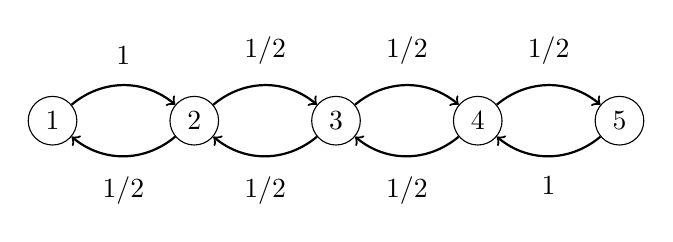
\begin{tikzpicture}[scale=0.9]
\node[draw, circle] (1) at (0,0) {$1$};
\node[draw, circle] (2) at (2,0) {$2$};
\node[draw, circle] (3) at (4,0) {$3$};
\node[draw, circle] (4) at (6,0) {$4$};
\node[draw, circle] (5) at (8,0) {$5$};

\path[draw,thick,->] (1) edge [bend left=40] node[font=\small,label=$1$] {} (2);
\path[draw,thick,->] (2) edge [bend left=40] node[font=\small,label=$1/2$] {} (3);
\path[draw,thick,->] (3) edge [bend left=40] node[font=\small,label=$1/2$] {} (4);
\path[draw,thick,->] (4) edge [bend left=40] node[font=\small,label=$1/2$] {} (5);

\path[draw,thick,->] (5) edge [bend left=40] node[font=\small,label=below:$1$] {} (4);
\path[draw,thick,->] (4) edge [bend left=40] node[font=\small,label=below:$1/2$] {} (3);
\path[draw,thick,->] (3) edge [bend left=40] node[font=\small,label=below:$1/2$] {} (2);
\path[draw,thick,->] (2) edge [bend left=40] node[font=\small,label=below:$1/2$] {} (1);

%\path[draw,thick,->] (1) edge [bend left=40] node[font=\small,label=below:$1$] {} (2);
\end{tikzpicture}
\end{center}

Марковтық тізбенің ықтималдылық үлестірімі 
-- $[p_1,p_2,\ldots,p_n]$ векторы, мұндағы
$p_k$ -- қазіргі күйіміз $k$ болуының ықтималдылығы. 
$p_1+p_2+\cdots+p_n=1$ формуласы әрдайым орындалады. 

Жоғарыдағы жағдайда бастапқы үлестірім -- $[1,0,0,0,0]$,
себебі біз бірінші қабаттан бастаймыз. Одан кейінгі үлестірім
$[0,1,0,0,0]$, себебі біз бірінші қабаттан тек екінші қабатқа
көше аламыз. Кейін біз төменге түсеміз не жоғарыға көтерілеміз,
демек келесі үлестірім -- $[1/2,0,1/2,0,0]$ және дәл солай 
кете береді.

Марковтық тізбедегі қадамдарды симуляциялаудың тиімді жолы
-- динамикалық бағдарламалауды қолдану.  
Динамикалық бағдарламалаудың идеясы -- 
ықтималдылық үлестірімін сақтай отырып,
әр қадамда барлық мүмкін болатын жолдарды қарастыру.  
Осы әдісті қолдана отырып, $m$ қадамдық кезуді $O(n^2 m)$ уақытта
симуляциялауымызға болады. 

Марковтық тізбенің ауысуларын ықтималдылық үлестірімді жаңартатын
матрица ретінде көрсетуге болады. Аталған жағдайға сәйкес төмендегідей матрица құрылады:

\[ 
 \begin{bmatrix}
  0 & 1/2 & 0 & 0 & 0 \\
  1 & 0 & 1/2 & 0 & 0 \\
  0 & 1/2 & 0 & 1/2 & 0 \\
  0 & 0 & 1/2 & 0 & 1 \\
  0 & 0 & 0 & 1/2 & 0 \\
 \end{bmatrix}.
\]

Ықтималдылық үлестірімін осы матрицаға көбейткенде, 
бір қадам өткеннен кейінгі ықтималдылық үлестірімді 
алатын боламыз. Мысалы $[1,0,0,0,0]$ ықтималдылық үлестірімнен
$[0,1,0,0,0]$ ықтималдылық үлестірімге келісі ретпен қозғалатын боламыз:

\[ 
 \begin{bmatrix}
  0 & 1/2 & 0 & 0 & 0 \\
  1 & 0 & 1/2 & 0 & 0 \\
  0 & 1/2 & 0 & 1/2 & 0 \\
  0 & 0 & 1/2 & 0 & 1 \\
  0 & 0 & 0 & 1/2 & 0 \\
 \end{bmatrix}
 \begin{bmatrix}
  1 \\
  0 \\
  0 \\
  0 \\
  0 \\
 \end{bmatrix}
=
 \begin{bmatrix}
  0 \\
  1 \\
  0 \\
  0 \\
  0 \\
 \end{bmatrix}.
\]

Матрицаның дәрежесін тиімді есептейтін болсақ, 
$m$ қадамнан кейінгі үлестірімді $O(n^3 \log m)$ уақытта
есептей аламыз. 

\section{Рандомизацияланған алгоритмдер}

\index{рандомизацияланған алгоритм}

Кейде ықтималдылыққа байланысы жоқ есептерді шығару
үшін кездейсоқтықты қолдануға болады. \key{Рандомизацияланған 
алгоритм} деп кездейсоқтыққа негізделген алгоритмді атаймыз. 

\index{Монте Карло алгоритмі}

\key{Монте Карло алгоритмі} –– кейде қате жауап
беретін рандомизацияланған алгоритм. Алгоритм пайдалы 
болу үшін жауаптың қате шығу ықтималдылығы төмен болуы 
тиіс.

\index{Лас Вегас алгоритмі}

\key{Лас Вегас алгоритмі} –– орындалу уақыты әртүрлі болатын және
әрдайым дұрыс жауап беретін алгоритм. Бұл жердегі мақсатымыз --
жоғары ықтималдылықпен тиімді алгоритмді жобалау. 

Біз төменде кездейсоқтықпен шығарылатын үш есепті қарастырамыз. 

\subsubsection{Реттік статистика}

\index{реттік статистика}

Жиымның $k$-\key{реттік статистикасы} --
жиымды сұрыптағаннан кейін $k$-позицияда тұратын
элемент. Кез келген реттік статистиканы 
$O(n \log n)$ уақытта жеңіл түрде есептеуге болады:
басында жиымды сұрыптаймыз, кейін $k$-элементті аламыз. 
Бірақ бір элементті табу үшін барлық жиымды сұрыптау 
шыныменде қажет пе?

Реттік статистиканы жиымды сұрыптамай, рандомизацияланған 
алгоритм арқылы да табуға болады екен. Мұндай алгоритмдердің біріне Лас Вегас алгоритмі типіне кіретін \key{quickselect} алгоритмі жатады\footnote{1961 жылы
Ч. А. Р. Хоар орташа есеппен тиімді екі алгоритмді, \index{quicksort} \index{quickselect}
жиымдарды сұрыптайтын \key{quicksort} \cite{hoa61a} және
реттік статистиканы табатын
\key{quickselect} \cite{hoa61b} алгоритмдерін жариялады.}.
Оның орындалу уақыты әдетте $O(n)$, бірақ ең жаман жағдайда $O(n^2)$ болады.

Алгоритм жиымның $x$ кездейсоқ элементін алады, сосын
$x$-тен кіші элементтерді жиымның сол жағына жылжытады, ал қалған барлық элементтерді жиымның оң жағына жылжытады.
Егер жиымда $n$ элемент бар болса, бұл $O(n)$ уақыт алады. 
Сол жағында $a$ элемент және оң жағында $b$ элемент бар делік.
Егер $a=k$ болса, $x$ элементі $k$-реттік статистика болады. 
Егер $a>k$ болса, біз $k$-реттік статистиканы рекурсивті
түрде сол жақтан іздейміз. Ал егер $a<k$ болса,
біз $r$-реттік статистиканы рекурсивті түрде оң жақтан
іздейтін боламыз, мұндағы $r=k-a$. Ізденіс солай элемент 
табылғанға дейін қайталана береді. 

% Assume that the left part contains $a$ elements
% and the right part contains $b$ elements.
% If $a=k$, element $x$ is the $k$th order statistic.
% Otherwise, if $a>k$, we recursively find the $k$th order
% statistic for the left part,
% and if $a<k$, we recursively find the $r$th order
% statistic for the right part where $r=k-a$.
% The search continues in a similar way, until the element
% has been found.

$x$ элементі кездейсоқ түрде алынған кезде 
жиымның өлшемі әр қадам сайын екіге бөлінеді.
Сондықтан $k$-реттік статистиканы табудың уақытша 
күрделілігі шамамен 
\[n+n/2+n/4+n/8+\cdots < 2n = O(n).\]

% When each element $x$ is randomly chosen,
% the size of the array about halves at each step,
% so the time complexity for
% finding the $k$th order statistic is about
% \[n+n/2+n/4+n/8+\cdots < 2n = O(n).\]

Алгоритм ең жаман жағдайда $O(n^2)$ уақытты қажет етеді,
өйткені $x$ саны жиымдағы ең кіші не ең үлкен сан болып 
таңдалынуы мүмкін және ол кезде $O(n)$ қадам жасау керек болады.
Бірақ ондай жағдайдың болуының ықтималдылығы өте төмен.
Сондықтан бұл тәжірибеде мүлдем кездеспейді. 

% The worst case of the algorithm requires still $O(n^2)$ time,
% because it is possible that $x$ is always chosen
% in such a way that it is one of the smallest or largest
% elements in the array and $O(n)$ steps are needed.
% However, the probability for this is so small
% that this never happens in practice.

\subsubsection{Матрицалардың көбейтіндісін тексеру}

\index{матрица көбейтіндісі}

Келесі есебіміз -- өлшемдері $n \times n$ болатын
$A$, $B$ және $C$ матрицаларға $AB=C$ орындалатынын 
\emph{тексеру}. 
Әрине бұл есепті шығару үшін 
$AB$ көбейтіндісін қайтадан (қарапайым алгоритм арқылы $O(n^3)$ уақытта) есептесек болады, бірақ жауапты тексеру 
қайтадан есептеуден әлдеқайда оңайырақ болуы керек
деген үміт бар. 

% Our next problem is to \emph{verify}
% if $AB=C$ holds when $A$, $B$ and $C$
% are matrices of size $n \times n$.
% Of course, we can solve the problem
% by calculating the product $AB$ again
% (in $O(n^3)$ time using the basic algorithm),
% but one could hope that verifying the
% answer would by easier than to calculate it from scratch.

Есепті уақытша күрделілігі $O(n^2)$ болатын
Монте Карло алгоритмі\footnote{Р. М. Фрейвалдс бұл алгоритмді 1977 жылы
жариялады \cite{fre77}, оны кейде \key{Фрейвалдс алгоритмі} деп те атайды.} 
арқылы шығаруға болады екен. Алгоритмнің идеясы -- қарапайым. 
Басында $n$ кездейсоқ элементтерден тұратын 
$X$ аламыз, сосын $ABX$ және $CX$ матрицаларын
есептейміз. Егер $ABX=CX$ орындалса, $AB=C$ деп
хабарлаймыз, әйтпесе $AB \neq C$ деп хабарлаймыз. 

% It turns out that we can solve the problem
% using a Monte Carlo algorithm\footnote{R. M. Freivalds published
% this algorithm in 1977 \cite{fre77}, and it is sometimes
% called \index{Freivalds' algoritm} \key{Freivalds' algorithm}.} whose
% time complexity is only $O(n^2)$.
% The idea is simple: we choose a random vector
% $X$ of $n$ elements, and calculate the matrices
% $ABX$ and $CX$. If $ABX=CX$, we report that $AB=C$,
% and otherwise we report that $AB \neq C$.

Алгоритмнің уақытша күрделілігі -- $O(n^2)$, 
себебі $ABX$ және $CX$ матрицалары
$O(n^2)$ уақытта есептелінеді. $ABX$ матрицасын
$A(BX)$ көрінісі арқылы тиімдірек есептеуімізге болады.
Осылайша екі $n \times n$ және $n \times 1$
матрицаларын көбейту ғана қажет болады. 

% The time complexity of the algorithm is
% $O(n^2)$, because we can calculate the matrices
% $ABX$ and $CX$ in $O(n^2)$ time.
% We can calculate the matrix $ABX$ efficiently
% by using the representation $A(BX)$, so only two
% multiplications of $n \times n$ and $n \times 1$
% size matrices are needed.

Алгоритмнің кемшілігі --
 $AB=C$ болуын кішкентай ықтималдылықпен қате баяндауында. 
% The drawback of the algorithm is
% that there is a small chance that the algorithm
% makes a mistake when it reports that $AB=C$.
Мысалы
\[
 \begin{bmatrix}
  6 & 8 \\
  1 & 3 \\
 \end{bmatrix}
\neq
 \begin{bmatrix}
  8 & 7 \\
  3 & 2 \\
 \end{bmatrix},
\]
бірақ
\[
 \begin{bmatrix}
  6 & 8 \\
  1 & 3 \\
 \end{bmatrix}
 \begin{bmatrix}
  3 \\
  6 \\
 \end{bmatrix}
=
 \begin{bmatrix}
  8 & 7 \\
  3 & 2 \\
 \end{bmatrix}
 \begin{bmatrix}
  3 \\
  6 \\
 \end{bmatrix}.
\]
Дегенмен тәжірибеде алгоритмнің қате орындау ықтималдылығы
төмен және сол ықтималдылықты бірнеше кездейсоқ
$X$ векторлармен тексеру арқылы одан сайын төмендете аламыз. 
% However, in practice, the probability that the
% algorithm makes a mistake is small,
% and we can decrease the probability by
% verifying the result using multiple random vectors $X$
% before reporting that $AB=C$.

\subsubsection{Графты бояу}

\index{бояу}

$n$ төбелер мен $m$ қырлардан тұратын граф берілген.
Біздің тапсырмамыз -- ең кемінде $m/2$ қырлардың 
шеттері әртүрлі түске ие болатындай етіп төбелерді бояу
жолын табу.  

% Given a graph that contains $n$ nodes and $m$ edges,
% our task is to find a way to color the nodes
% of the graph using two colors so that
% for at least $m/2$ edges, the endpoints 
% have different colors.
Мысалы, төмендегі графта
\begin{center}
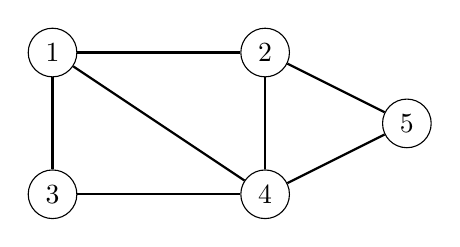
\begin{tikzpicture}[scale=0.9]
\node[draw, circle] (1) at (1,3) {$1$};
\node[draw, circle] (2) at (4,3) {$2$};
\node[draw, circle] (3) at (1,1) {$3$};
\node[draw, circle] (4) at (4,1) {$4$};
\node[draw, circle] (5) at (6,2) {$5$};

\path[draw,thick,-] (1) -- (2);
\path[draw,thick,-] (1) -- (3);
\path[draw,thick,-] (1) -- (4);
\path[draw,thick,-] (3) -- (4);
\path[draw,thick,-] (2) -- (4);
\path[draw,thick,-] (2) -- (5);
\path[draw,thick,-] (4) -- (5);
\end{tikzpicture}
\end{center}
жарамды бояулардың бірі осындай болмақ:
% a valid coloring is as follows:
\begin{center}
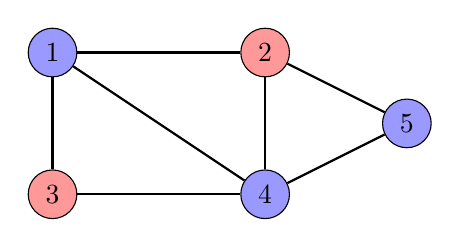
\begin{tikzpicture}[scale=0.9]
\node[draw, circle, fill=blue!40] (1) at (1,3) {$1$};
\node[draw, circle, fill=red!40] (2) at (4,3) {$2$};
\node[draw, circle, fill=red!40] (3) at (1,1) {$3$};
\node[draw, circle, fill=blue!40] (4) at (4,1) {$4$};
\node[draw, circle, fill=blue!40] (5) at (6,2) {$5$};

\path[draw,thick,-] (1) -- (2);
\path[draw,thick,-] (1) -- (3);
\path[draw,thick,-] (1) -- (4);
\path[draw,thick,-] (3) -- (4);
\path[draw,thick,-] (2) -- (4);
\path[draw,thick,-] (2) -- (5);
\path[draw,thick,-] (4) -- (5);
\end{tikzpicture}
\end{center}
Жоғарыдағы граф 7 қырдан тұрады және 5-еуінің
шеттері әртүрлі түске ие, демек
бұл бояу жарамды деп саналады.
% The above graph contains 7 edges, and for 5 of them,
% the endpoints have different colors,
% so the coloring is valid.

Есепті жарамды бояуды тапқанша дейін кездейсоқ түрде бояйтын 
Лас Вегас алгоритмі арқылы шығаруға болады. Кездейсоқ
бояуда әр төбенің түсі $1/2$ ықтималдылықпен 
тәуелсіз түрде таңдалады. 

% The problem can be solved using a Las Vegas algorithm
% that generates random colorings until a valid coloring
% has been found.
% In a random coloring, the color of each node is
% independently chosen so that the probability of
% both colors is $1/2$.

Кездейсоқ бояуда бір қырдың шеттері бірдей емес түске 
ие болуының ықтималдылығы -- $1/2$. Демек қырлардың
шеттері бірдей емес түске ие болуының математикалық
күтімі -- $m/2$. Кездейсоқ бояу жарамды деп күтілгендіктен,
іс жүзінде жарамды бояуды тез табатын боламыз.

% In a random coloring, the probability that the endpoints
% of a single edge have different colors is $1/2$.
% Hence, the expected number of edges whose endpoints
% have different colors is $m/2$.
% Since it is expected that a random coloring is valid,
% we will quickly find a valid coloring in practice.

